\section{ Machine learning}

According to Arthur Samuel (qtd. in Geron \cite{geron}) machine learning is a field of study that gives computers the ability to learn without being explicitly programmed.
This ability to learn is the property of various machine learning algorithms.
We will be using the terms "machine learning" and "learning" interchangeably. 
To learn, these learning algorithms need to be trained on a collection of examples of some phenomenon\cite{burkovml}. 
These collections are called \textbf{datasets} and can be generated artificially or collected in nature.

To better understand how ML approach can solve problems, we can examine an example application.
Let us say that we would like to build a system that can predict a type of animal movement based on accelerometer data.
To train its learning algorithm, also known as a \textbf{model}, we need to train it on a dataset that contains accelerometer measurements of different types of movement, such a walking, running, jumping and standing still.
Input to the system could be either raw measurements from all three axis or components extracted from raw measurements such as RMS, spectral power, peak frequency and/or peak amplitude. 
These inputs are also known as \textbf{features}, they are values that describe the phenomenon being observed\cite{burkovml}. 
The output of the system would be a predicted type of movement.
Although we would mark each example of measurement data what type of movement it represents, we would not directly define the relationship between the two.
Instead, we would let the model figure out the connection by itself, through the process of training.
The trained model should be general enough so it can correctly predict the type of movement on unseen accelerometer data.

There exists a large variety of different learning algorithms. 
We can broadly categorize them in several ways, one of them depends on how much supervision the learning algorithm needs in the training process. 
Algorithms like K-nearest neighbors, linear and logistic regression, support vector machines fall into the category of supervised learning algorithms.
Training data that is fed into them includes solutions, also known as \textbf{labels}\cite{geron}.
Described above example is an example of a supervised learning problem.

Algorithms like k-Means, Expectation Maximization, Principal Component Analysis fall into the category of unsupervised learning algorithms.
Here training data is unlabeled, algorithms are trying to find similarities in data by itself\cite{geron}.
There exist other categories such as semi-supervised learning which is a combination of the previous two and reinforcement learning, where model acts inside the environment according to learned policies\cite{geron}.

Neural networks, algorithms inspired by neurons in human brains\cite{geron}\cite{cs231n}, can fall into either of categories. 
They are appropriate for solving complex problems like image classification, speech recognition, and autonomous driving, but they require a large amount of data and computing power for training.
They fall into the field of deep learning, which is a sub-field of machine learning.

Training of ML models is computationally demanding and is usually done on powerful servers or computers with dedicated graphic processing units to speed up training time.
After a model has been trained, data can be fed in and prediction is computed. 
This process is also known as \textbf{inference}.
The inference is computationally less intensive compared to the training process, so with properly optimized models, we can run inference on personal computers, smartphones, tablets, and even directly in internet browsers.


\subsection{ General machine learning workflow}

There are several steps in ML workflow that need to happen to get from an idea to a working ML based system, this is represented in Figure \ref{ml_workflow}.

\begin{figure}[ht]
        \centering
        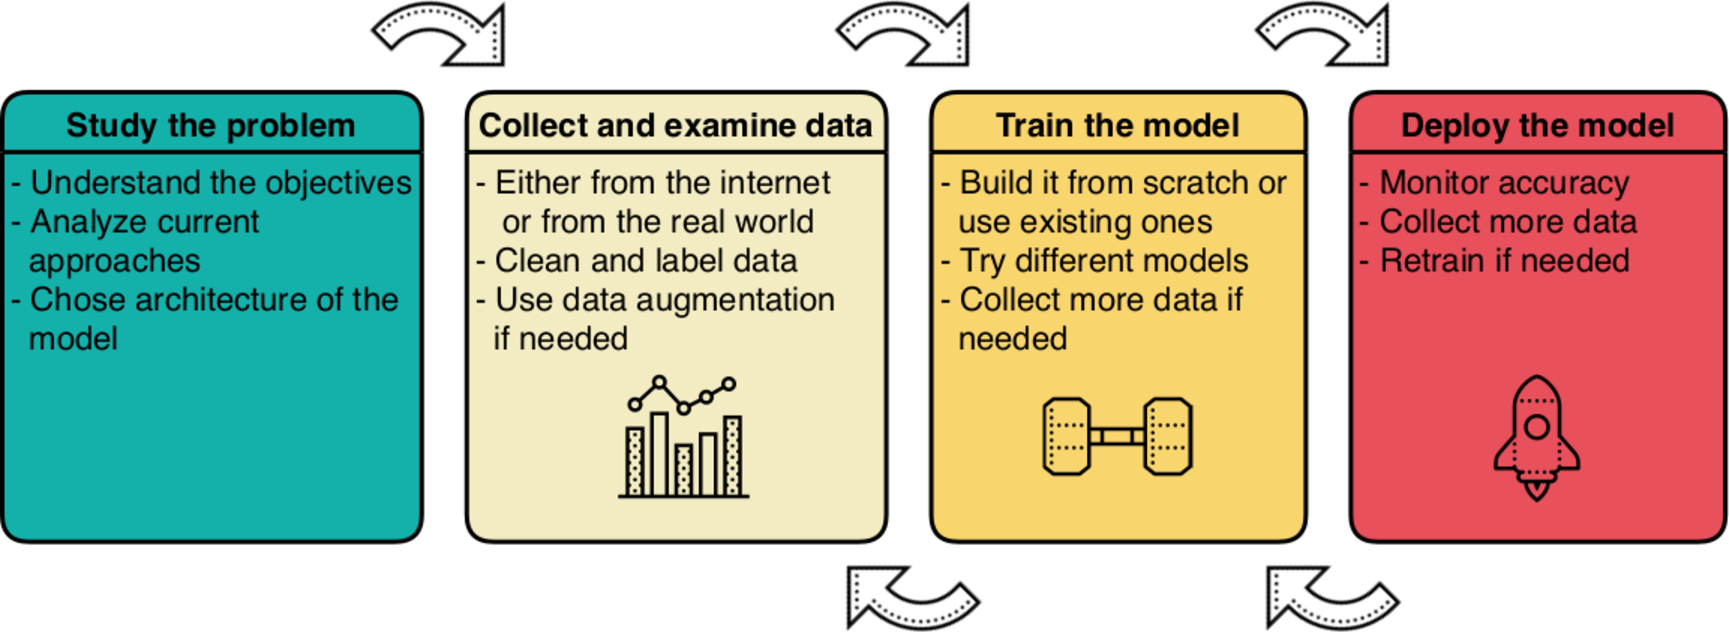
\includegraphics[width=1.0\linewidth]{ml_workflow.pdf} 
        \caption[Workflow diagram of solving a generic machine learning problem.] {Workflow diagram of solving a generic machine learning problem. Icons source:\cite{icons}}
        \label{ml_workflow}
\end{figure}

First, the problem has to be studied, it has to be understood what are objectives, what are current solutions and which approach should be used. 
Here we decide on the rough type of the ML model that we will use, based on the problem.
In the second step we collect and clean up data.
We should always strive to collect a large amount of quality and diverse data that represents real world phenomenon.
Collecting that kind of data can be hard and expensive, but we can use various tools, such as data augmentation or data synthesis, thus increasing data size and variety.
Sometimes data is not collected by us, in that case we should examine it and extract information that we need.
Third, we train the ML model.
We might create something from scratch or use an existing model. 
We can train several different types of models and chose the one that performs the best.
To achieve the desired accuracy steps two and three can be repeated many times.
In step four we deploy our model and monitor its accuracy. 
We should always collect new data and retrain the model, if accuracy drops.


\subsection{ Machine learning on embedded devices} \label{ml_on_embedded}

Machine learning on embedded devices is an emerging field, which nicely coincides with the Internet of things.
Resources about it are limited, especially when compared to the wast number of resources connected with machine learning on computers or servers.
Most of the information about it can be found in form of scientific papers, blog posts and machine learning framework documentation\cite{hello_edge}\cite{tflite_risc-v}\cite{pete_tiny}.

Running learning algorithms directly on embedded devices comes with many benefits.
\textbf{Reduced power consumption} is one of them.
In most IoT applications devices send raw sensor data over a wireless network to the server, which processes it either for visualization or for making informed decisions about the system as a whole. 
Wireless communication is one of the more power hungry operations that embedded devices can do, while computation is one of more energy efficient\cite{pete_tiny}.
For example, a Bluetooth communication might use up to 100 milliwatts, while MobileNetV2 image classification network running 1 inference per second would use up to 110 microwatts\cite{pete_tiny}
As deployed devices are usually battery powered, it is important to keep any wireless communication to a minimum, minimizing the amount of data that we send is paramount.
Instead of sending everything we capture, is much more efficient to process raw data on the devices and only send results.

Another benefit of using ML on embedded devices is \textbf{decreased latency time}.
If the devices can extract high-level information from raw data, they can act on it immediately, instead of sending it to the cloud and waiting for a response. 
Getting a result now takes milliseconds, instead of seconds.

Such benefits do come with some drawbacks.
Embedded devices are a more resource constrained environment when compared to personal computers or servers.
Because of limited processing power, it is not feasible to train ML models directly on microcontrollers.
Also it is not feasible to do online learning with microcontrollers, meaning that they would learn while being deployed.
Models also need to be small enough to fit on a device. 
Most general purpose microcontrollers only offer several hundred kilobytes of flash, up to 2 megabytes.
For comparison, MobileNet v1 image classification model, optimised for mobile phones, is 16.9 MB in size\cite{daniel_edgeimpulse}.
To make it fit on a microcontroller and still have space for our application, it would have to be simplified.

The usual workflow, while developing machine learning models for microcontrollers, is to train a model on training data on a computer. 
When we are satisfied with the accuracy of the model we quantize it and convert it into a format understandable to our microcontroller.
This is further described in section \ref{tflite_quant}.

\section{ Neural networks}\label{neural_networks_section}

Although the first models of neural networks (NN) were presented in 1943 (by McCulloch and Pitts)\cite{geron} and hailed as the starting markers of the artificial intelligence era, it had to pass several decades of research and technological progress before they could be applied to practical, everyday problems.
Early models of NNs, such as the one proposed by McCulloch and Pitts were inspired by how real biological neural systems work. 
They proved that a very simple model of an artificial neuron, with one or more binary inputs and one binary output, is capable of computing any logical proposition when used as a part of a larger network\cite{geron}.

To learn how NNs work we can refer to Figure \ref{neuron_model}, which shows a generic version of an artificial neuron.
\newline

\begin{figure}[ht] 
    \begin{subfigure}[b]{0.5\textwidth}
        \centering
        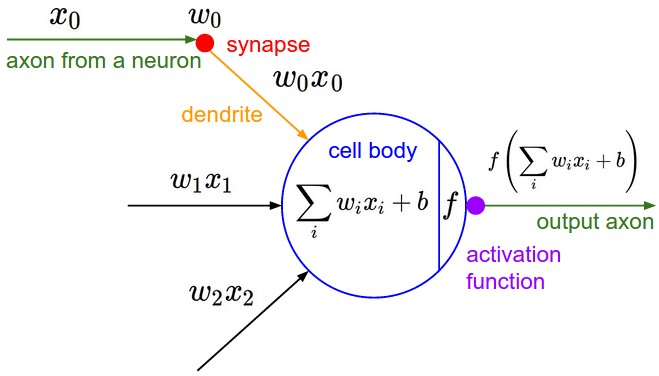
\includegraphics[width=1.0\linewidth]{neuron_model.jpeg} 
        \caption{Artificial neuron}
        \label{neuron_model}
    \end{subfigure}
    \unskip\ \vrule\ 
    \begin{subfigure}[b]{0.5\textwidth}
        \centering
        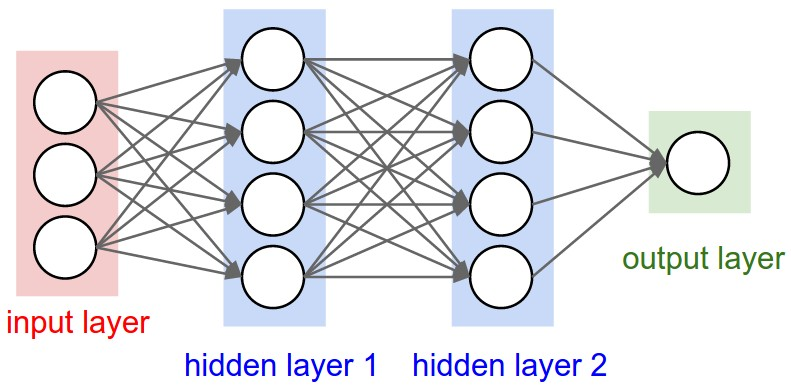
\includegraphics[width=1.0\linewidth]{neural_net.jpeg} 
        \caption{ 3-layer neural network}
        \label{neural_net}
    \end{subfigure}
    
    \caption[Mathematical model of artificial neuron and fully connected 3-layer neural network.]{(a) Mathematical model of an artificial neuron, similarities with biological neurons can be seen. (b) Fully connected 3-layer neural network. Image source: \cite{cs231n}}
    \label{neural}
\end{figure}

Neuron takes several inputs, multiplies each input with its \textbf{weight} and sums them up.
It adds to the sum the \textbf{bias} term and then applies an activation function.

NNs consist of many neurons, which are organized into \textbf{layers}.
Neurons inside the same layer do not share any connections, but they connect to layers before and after them.
First layer is known as \textbf{input} layer and last one is known as \textbf{output} layer. 
Any layers between are said to be \textbf{hidden}. 
In Figure \ref{neural_net} we can see a neural network with an input layer with three inputs, two hidden layers with four neurons each and an output layer with just one neuron.
If all inputs of neurons in one layer are connected to all outputs from the previous layer, we say that a layer is \textbf{fully connected} or \textbf{dense}, Figure \ref{neural_net} is an example of one.
NNs with many hidden layers fall into the category of deep neural networks (DNN).


\subsection{ Activation functions}

Activation functions introduce non-linearity to a chain of otherwise linear transformations, which enables ANNs to approximate any continuous function\cite{geron}.
There are many different kinds of activation functions as seen on Figure \ref{activation_functions}, such as sigmoid function and rectified linear activation function (ReLu).
A sigmoid function was commonly used in the past, as it was seen as a good model for a firing rate of a biological neuron: 0 when not firing at all and 1 when fully saturated and firing at maximal frequency\cite{cs231n}.
It takes a real number and squeezes it into a range between 0 and 1.
It was later shown that training NNs with sigmoid activation function often hinders the training process as saturated outputs cut off parts of networks, thus preventing the training algorithm from reaching all neurons and correctly configuring the weights\cite{cs231n}.
It has since fallen out of practice and is nowadays replaced by ReLu or some other activation function.

\begin{figure}[ht!]
        \centering
        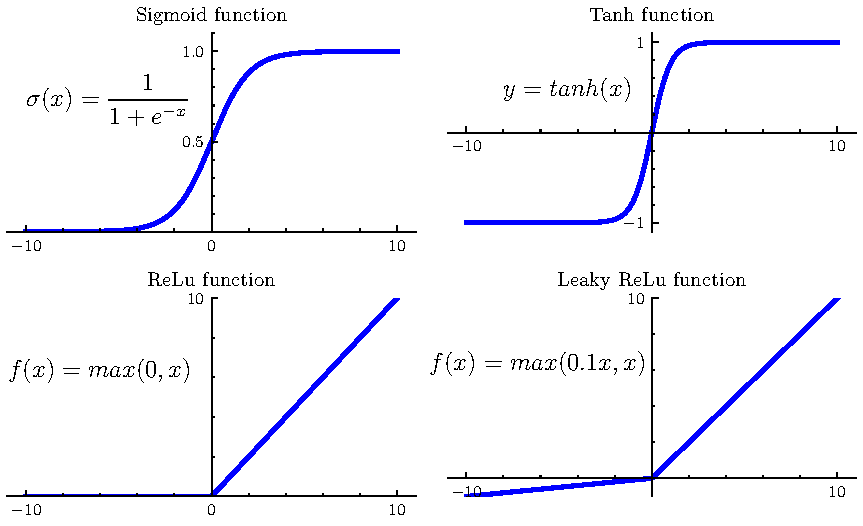
\includegraphics[width=1.0\linewidth]{activation_func.pdf} 
        \caption{Different activation functions and their equations.}
        \label{activation_functions}
\end{figure}


Another commonly used activation function is a softmax function (seen in \ref{softmax_equ}, which is takes a vector as an input, computes an exponential of every element inside it and divides that with the sum of exponents of all elements\cite{geron}
The end results is that softmax function transforms vector of values into a vector of probabilities.
Softmax is usually used as an activation in a last layer of a classifier network. 

\begin{equation}\label{softmax_equ}
    \sigma(y_i) = \frac{e^{y_i}}{\sum_{j=1}^{K}e^{y_j}}\;\;\;\text{for}\;\;i\;=\;1,\cdots,K\;\;\text{and}\;\;y=(y_1,\cdots,y_k)\in\mathbb{R}^K
\end{equation}

Where:

$y$ - Input vector

$K$ - Number of elements in input vector

$\sigma(y_i)$ - Computed probability of i-th element in input vector 


\subsection{ Backpropagation}

Training of neural networks is done with a training algorithm, known as \textbf{backpropagation}.
As mentioned before, we train the neural network by showing it a large amount of training data with labels.
At the start of the training phase, all weights and biases are set to randomly small values.
During each training step, a neural network is shown a small batch of training data. 
Each instance is feed into NN and the final output label is calculated.
This is known as \textbf{forward pass}, which is the same as making predictions, except that intermediate results from each neuron in every layer are stored.
Calculated output is compared to an expected one using a \textbf{loss} (also known as \textbf{cost}) function.
The loss function returns a single value, which tells us how badly is our NN performing, the higher it is, the worse is our NN performing.
The goal is to minimize the loss function, thus increasing the accuracy of our NN.
In the context of multivariable calculus, this means that we have to calculate the negative gradient of weights and biases which will tell us in which direction we have to change each weight and bias so that value of loss function decreases. 

Doing this for all weights and biases at the same time would be complicated, so the backpropagation algorithm does this in steps.
After computing the loss function algorithm analytically calculates how much each output connection contributed to the loss function (essentially local gradient) with the help of previously stored intermediate values.
This step is recursively done for each layer until the first input layer is reached.
At that moment algorithm knows in which direction should each weight and bias change so that value of the loss function lowers.
A procedure known as a \textbf{Gradient Descent} is then performed.
All local gradients are multiplied with a small number known as \textbf{learning rate} and then subtracted from all weights and biases.
This way in each step we slowly change weights and biases in the right direction, while minimizing a loss function.
Gradient Descent is not only used when training neural networks but also when training other ML algorithms.

We do not have to execute a backpropagation algorithm for each training instance, instead we can calculate predictions for a small set of training data, calculate the average loss function and then apply backpropagation.


\subsection{ Convolutional neural networks}

Convolutional neural networks (CNN) are a kind of neural networks that work especially well with image data.
Like NNs they have found inspiration in nature, in their case visual cortex of the brain.\footnotemark
\footnotetext{Scientists Weisel and Hubel showed that different cells in the primary visual cortex of a cat responded differently to different visual stimuli\cite{cs231n}.
Some were activated when shown a horizontal line in a specific location, some were activated by vertical lines.
More complex cells responded to boxes, circles and so on.
CNNs also detect simpler shapes first and use them to detect more complex ones later.}

In Figure \ref{convnet} we can see an example of CNN which takes an image of a car as an input and outputs probability results in five different classes.
\newline

\begin{figure}[ht]
        \centering
        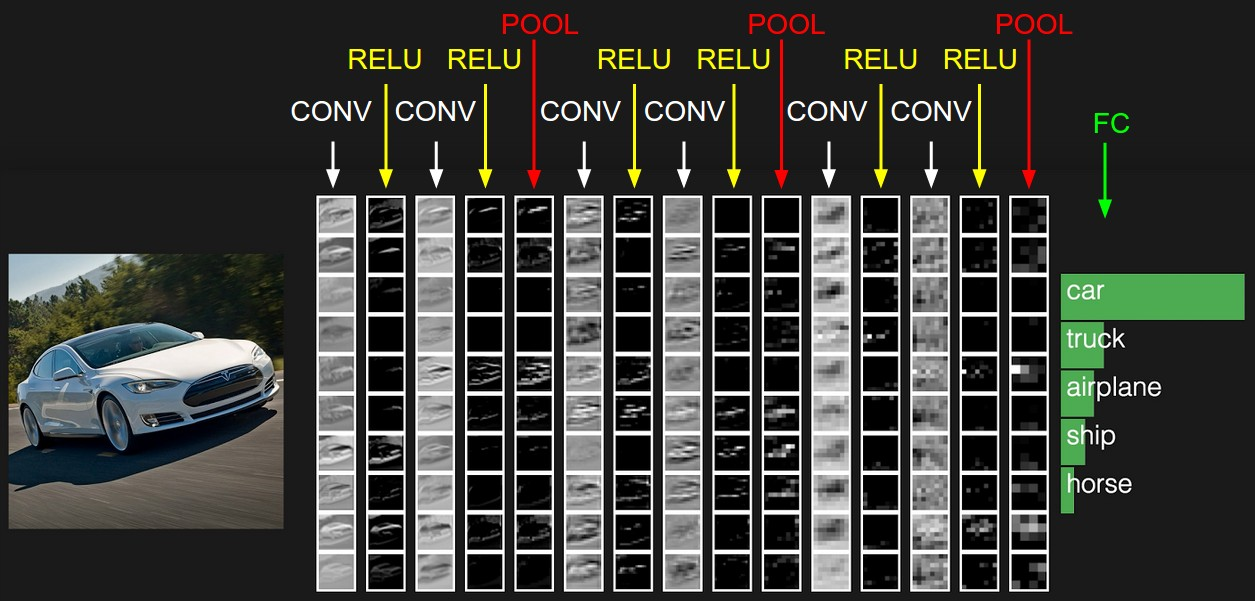
\includegraphics[width=1.0\linewidth]{convnet.jpeg} 
        \caption[Structure of a convolutional neural network.]{Structure of a convolutional neural network. Image source:\cite{cs231n}}
        \label{convnet}
\end{figure}

Specific to CNNs are two different types of layers, \textbf{convolutional} layers and \textbf{pooling} layers.
Each convolutional layer detects some sort of shapes, first ones detect different kinds of edges, later ones detect more complex shapes and objects, like wheels, legs, eyes, ears.
Pooling layers downsample the data in the spatial dimension, thus decreasing the number of parameters and operations needed in CNN.
After a few alternating pairs of convolutional and pooling layers, the output of the last pooling layer is flattened out into one dimensional vector and feed into fully connected NN which produces probability results in given classes.

It makes sense to explain how convolutional and pooling layers work in greater detail as this will be important later when we will be designing our CNN models in section \ref{cnn_ref}.


\subsubsection{ Convolutional layers}

Data that CNNs operate on are 3 dimensional matrices, where width and height correspond to image resolution and depth corresponds to the number of color channels, 3 for colorful images (red, green, blue) and 1 for greyscale.
When speaking about these matrices we will refer to them as volumes.

Convolution layers perform dot products between input volume and several \textbf{filters} or \textbf{kernels} to produce output volume.
In these layers, filters are configured through the training phase.
We can see a concrete example in Figure \ref{conv1}.
2D filter with size 2 x 2 covers a part of the input volume, over which element-wise multiplication is computed, elements are summed and the result is written into the first element of output volume.

\begin{figure}[ht] 
    \centering
    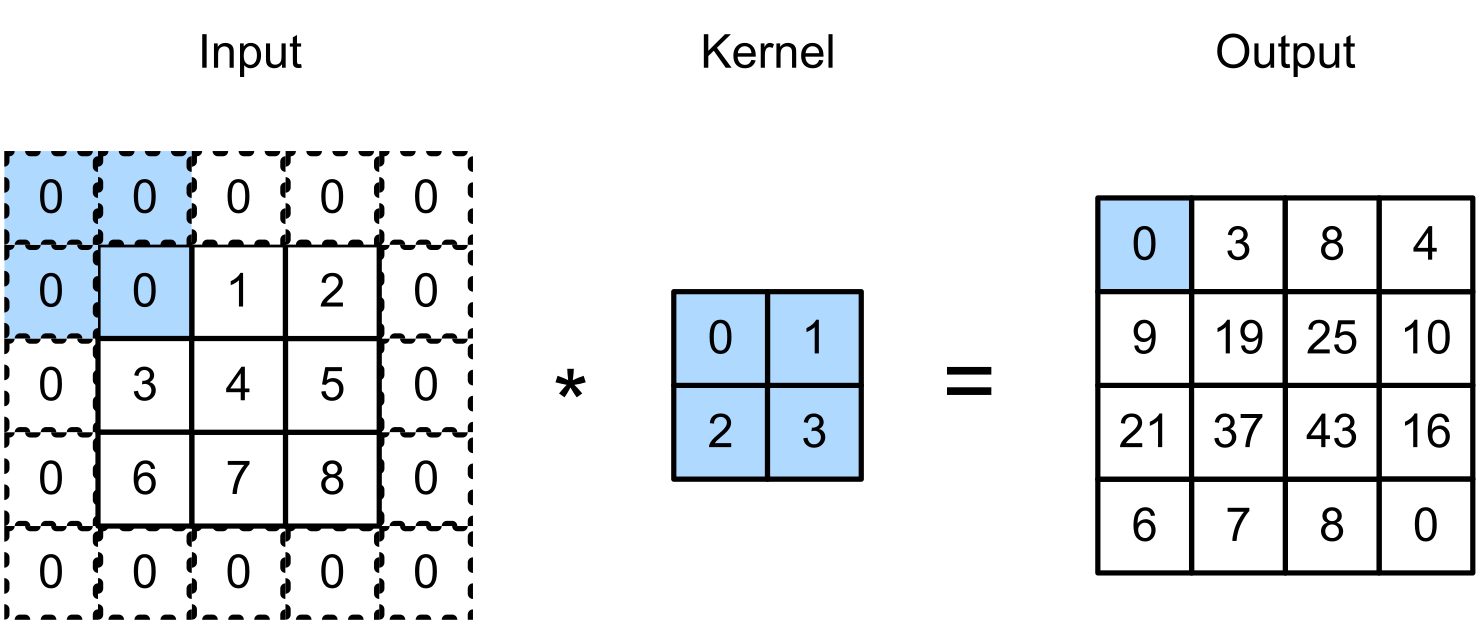
\includegraphics[width=0.75\linewidth]{conv1.png} 
\caption[Dot product operation between filter and zero-padded input matrix.] {Dot product operation between filter and zero-padded input matrix. Image sources: \cite{conv_layer_img}}
    \label{conv1}
\end{figure}

The filter then moves a fixed distance or \textbf{stride} and the process is repeated.
It is important to note that although we can choose the width and height of the filter, the depth of the filter is always equal to the depth of the input volume.
If the depth is larger than one then dot products are done for each 2D matrix in depth dimension separately and then element-wise sum operation between these matrices is performed.
To avoid losing information from the image pixels that are on the edges (as they would be included in dot products fewer times compared to central ones) we often pad input images with zeros.

The size of output volume depends on several factors as seen in \ref{size_eq}.

\begin{equation}\label{size_eq}
V_{o} = (V_{i} - F + 2P) / S + 1
\end{equation}

Where:

$V_{i}$ - Input volume size, only width or height

$V_{o}$ - Output volume size, only width or height

$F$ - Filter or receptive field size

$P$ - Amount of zero padding used on the border

$S$ - Stride length

If we examine the example in Figure \ref{conv1} we can see that input with a size 3 x 3, stride 1, padding 1 and filter with a size 2 x 2 produces output with size a 4 x 4.

The depth of output volume is equal to the number of filters used in the convolutional layer as seen in Figure \ref{conv2}, it is a norm that a single convolutional layer uses a large number of filters to produce a deep output volume\cite{cs231n}.
It is also common to set padding, stride and filter size so that the width and height of input volume are preserved.
This prevents the information at the edges to be lost too quickly\cite{cs231n}.


\begin{figure}[ht] 
    \centering
    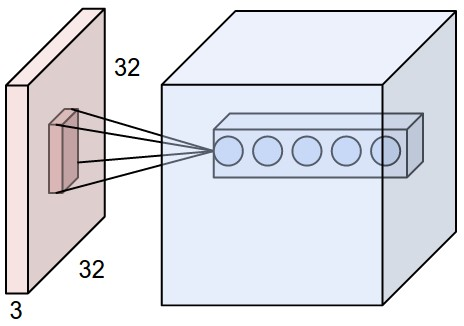
\includegraphics[width=0.5\linewidth]{conv2.jpeg} 
\caption[Convolutional layer with five different filters.] {Convolutional layer with five different filters. Image sources: \cite{conv_layer_img}\cite{cs231n}}
    \label{conv2}
\end{figure}

At the end of the convolutional layer output volume is fed into neurons similar to one described in section \ref{neural_networks_section}. 
All elements in the same depth are affected by the same bias term and fed into the activation function.
In this step, the size of the volume is preserved.

\subsubsection{ Pooling layers}

Polling layers perform the downsampling of input volumes in width and height dimensions.
This is done by sliding a filter of fixed size over input and doing MAX operation on elements that filter covers, only the largest value element is copied into output (Figure \ref{pool_layer}).
Pooling is done on each depth slice separately of other slices, so depth size is preserved through the layer.

\begin{figure}[ht] 
    \begin{subfigure}[b]{0.5\textwidth}
        \centering
        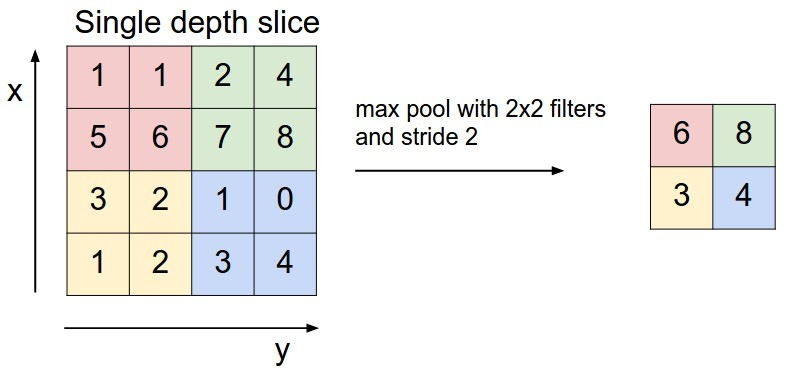
\includegraphics[width=1.0\linewidth]{pool1.jpeg} 
        \caption{Max pooling operation}
        \label{pool1}
    \end{subfigure}
    \unskip\ \vrule\ 
    \begin{subfigure}[b]{0.5\textwidth}
        \centering
        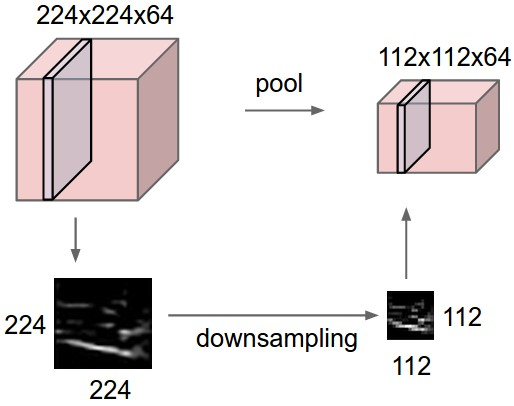
\includegraphics[width=1.0\linewidth]{pool2.jpeg} 
        \caption{ Effect of polling on input dimensions}
        \label{pool2}
    \end{subfigure}
    \caption[Polling layer.] {Pooling layer. Image source: \cite{cs231n}}
    \label{pool_layer}
\end{figure}

It is common to select pool size 2 x 2 and stride 2.
Like this, inputs are downsampled by two in height and width dimensions, discarding 75 \% activations.
Pooling layers therefore reduce the number of activations and prepare them to be flattened out and fed into a fully connected layer.

\section{ TensorFlow}

TensorFlow is a free and open-source framework for numerical computation.
It is particularly suited for large-scale machine learning applications\cite{geron}.
It started as a proprietary project developed by a Google Brain team at Google in 2011 and became open-source in late 2015.
It is used in many of Google's products such as Gmail, Google Cloud Speech and Google Search.

TensorFlow gives programmers tools for creating and training ML models, without needlessly diving into specifics of computing neural networks.
Programmers can write high level code in Python API, which calls highly efficient C++ code.
When using TensorFlow the hardest part of an ML project is usually data preparation.
After that is done, the creation of an ML model, its training and evaluation can be done in a few lines of Python code.

TensorFlow also supports Keras high level API for building ML models. 
Keras is a Python library that functions as a wrapper for TensorFlow.
When building ML models developers can use Keras Sequential API, where each layer in a model is represented as one line of code.
Users do not need to care about connections between the layers, they only need to choose the type of layer (convolutional, max pool, fully connected), its size and few other specific parameters.
Sequential API is used most of the time, if a finer level of control is needed TensorFlow provides low level math operations as well.

And finally, TensorFlow's trained output model is portable\cite{geron}.
Models can be trained in one environment and executed in another.
This means that we can train our model by writing Python code on a Linux machine and execute it with Java on a Android device.
This last functionality is important for running ML models on microcontrollers.

\subsection{ TensorFlow Lite for Microcontrollers} \label{tflite_quant}

TensorFlow Lite (TFLite) is a set of tools and libraries that enable running ML inferences on constrained devices\cite{tensorflow_github}.
It provides support for Android and iOS devices, and embedded Linux.
TensorFlow Lite for Microcontrollers (TFLite Micro) is a recent port of TFLite (as of mid 2019), dedicated to running ML models on microcontrollers.
TFLite itself provides API in different languages, such as Java, Swift, Python and C++.
TFLite Micro uses C++ API, specifically C++11, which reuses a large part of the general TensorFlow codebase.

TFLite Micro library does not require any specific hardware peripherals, which means that the same C++ code can be compiled to run on a microcontroller or a personal computer with minimal changes.
Users are only expected to implement their version of \verb|printf()| function.
As microcontroller binaries are usually quite big, flashing firmware to a microcontroller is a time consuming procedure.
It makes sense to first test and debug the program that includes only ML inference specific code on a personal computer, before moving on to a microcontroller to save time.
Implementation of test setup is described in TODO ADD REFERENCE.

TFLite Micro library is publicly available as a part of a much larger TensorFlow project on GitHub\cite{tensorflow_github}.
To use the library for embedded development the whole project has to be cloned from the GitHub.
The TensorFlow team provides users with several example projects that have been ported to several different platforms such as Mbed, Arduino, OpenMV and ESP32.
Example projects show how to use TFLite API while showcasing different ML applications: motion detection, wake word detection and person detection.

Is important to know that TFLite is just an extension of the existing TensorFlow project.
General steps for creating a trained ML model are still the same as seen in Figure \ref{ml_workflow}, although we have to be aware of some details.
Figure \ref{micro_workflow} shows all steps that are needed to prepare an ML model for running on a microcontroller.

\begin{figure}[ht] 
    \centering
    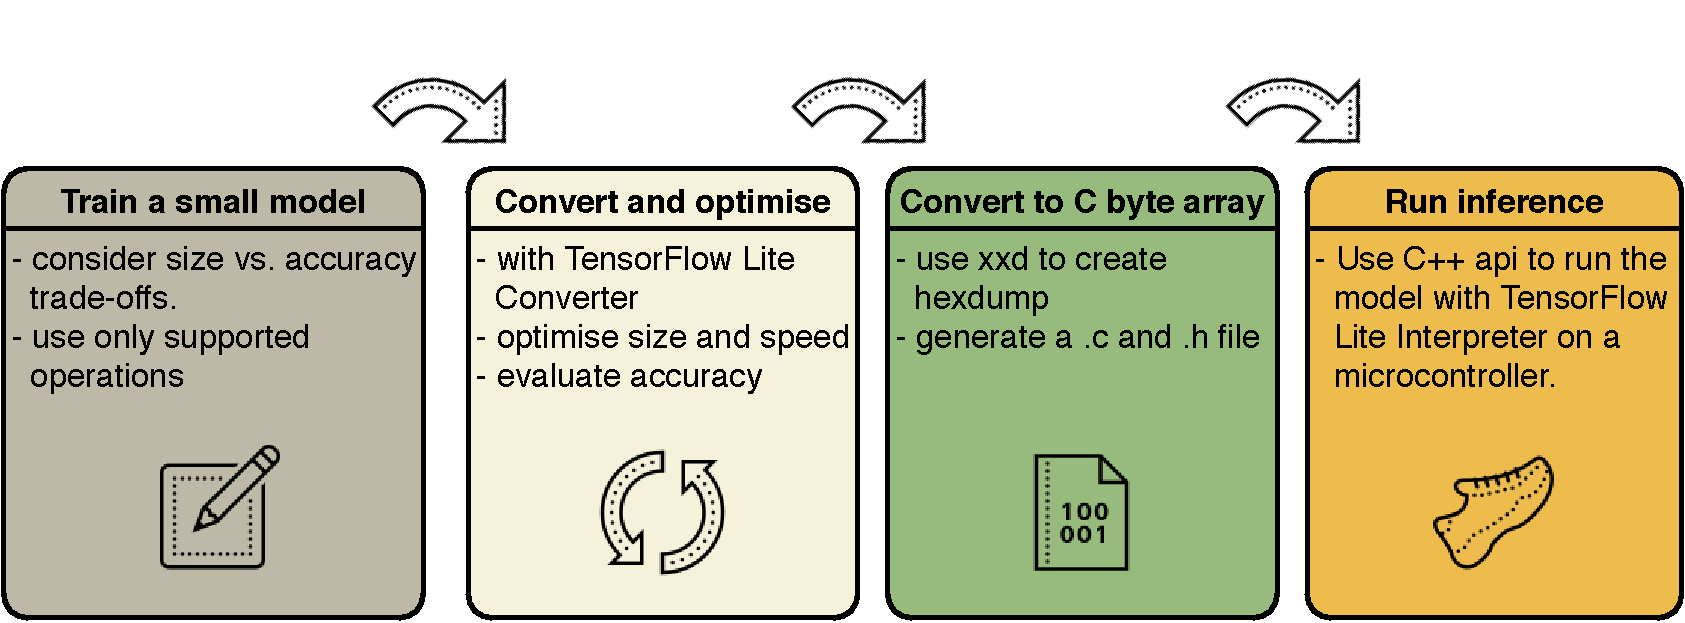
\includegraphics[width=1.0\linewidth]{micro_workflow.pdf} 
    \caption[Workflow of preparing a ML model for an inference on a microcontroller.]{Workflow of preparing a ML model for an inference on a microcontroller. Icons source:\cite{icons}}
    \label{micro_workflow}
\end{figure}

We start with a small but inaccurate model that can still accomplish the basic criteria that our objective demands.
When the end of this workflow process is reached and we made sure that the model can fit into a flash memory area of our target microcontroller, we can start training more complex models to increase accuracy.
We are allowed to use only operations that have supported implementations on microcontrollers.
This is usually not a restriction as many of them are supported.

The model that is created is usually quite big and needs to be converted with the TensorFlow Lite Converter tool.
This tool provides a non-optimized conversion and several different optimized conversions.

To import and use the optimized model, we need to convert it into binary format, which is done with the command line tool xxd.
The model is then ready to be executed on a microcontroller, we can run it and process the results.
Accuracy will be the same as compared to running the same .tflite model on a personal computer, but execution time will naturally be different.
If needed we can tweak the model parameters, train a new model and repeat the described workflow again.


\subsubsection{ Post-training quantization}

By using quantization optimization we approximate floating-point numbers in a different format, usually with 8-bit integers.
When computing neural networks we can quantize weights, biases and intermediate values output by separate neurons. 
Quantization has a dramatic effect on the size of the model and its execution speed.
By changing 32-bit floating-point numbers with 8-bit integers size decreases by a factor of 4.
Floating-point math is by nature slow to compute, many microcontrollers do not even have a floating-point unit.
In comparison integer math is faster to compute, therefore quantized models are executed faster.
Model accuracy decreases after using quantization, but usually for less than a percent.
 

\section{ IoT and wireless technologies}

Internet of things, or IoT, is a system of uniquely identifiable devices, which communicate with each other or other systems over wireless networks\cite{IoT}.
A device or a thing is a battery powered embedded system such as smart watch, heart monitor, or animal tracker which would transmit collected sensor data to an IoT gateway, which would relay the data over to the cloud.
This data can then be analyzed and displayed in such fashion which would provide businesses or users with valuable information.
Examples of this would be tracking the energy consumption of machines in factories, monitoring conditions of crops in agriculture, or monitoring locations of endangered species in African conservation parks.

An important part of IoT system is a wireless network that is used to transport data from edge devices to gateways or directly to the internet.
The choice of a wireless network is highly dependent on a type of a problem an IoT solution is trying to solve.
Factors such as required battery life, amount of data being sent, the distance that data has to travel and environment conditions of the edge device itself are important.

Because our early detection system demands a decent battery life of several months and needs to send a small amount of data over one or two kilometers we will focus on wireless technologies such as NB-IoT, Sigfox and LoRa.

Narrowband IoT or NB-IoT is a radio technology standard developed by 3GPP standard organization\cite{lora_nbiot}.
NB-IoT was made specifically with embedded devices in mind, it has a range of to 15 \si{\kilo\meter} and it has deep indoor penetration\cite{lora_nbiot}.
Compared to Sigfox and LoRa it has better latency and higher data rate, but also higher power consumption\cite{lora_nbiot_sigfox}.
However it is unsuitable for our use case as it operates on the network provided by the cellular base towers, which is inconvenient as the mobile connection in Assam, India can be inconsistent\cite{wildlabs-elephants}.

Sigfox is a radio technology developed by the company of the same name that operates on an unlicensed industrial, scientific and medical (ISM) radio band.
In many views it is similar to LoRa, as it has the comparative range and power consumption\cite{lora_nbiot_sigfox}.
However, there are a few important differences.
Although Sigfox modules are a bit cheaper when compared to Lora modules, each message is paid, devices are limited to 12 bytes per uplink, 140 uplinks per day and only 4 downlinks are available per day.
Sigfox devices can also only communicate with base stations, installed by the Sigfox company\cite{lora_nbiot_sigfox}.
This means that users can not build their own network and are dependent on the coverage provided by Sigfox.

This leaves us with Lora protocol which covers our use case from points of long range, low power consumption and ability to set up our own network. 


\subsection{ LoRa and LoRaWAN}

LoRa (Long Range) is a physical layer protocol that defines how information is modulated and transmitted over the air\cite{lora_article}\cite{lora_nbiot}.
The protocol is proprietary and owned by a semiconductor company Semtech, who is the sole designer and manufacturer of Lora radio chips in the world.
LoRa protocol uses a modulation similar to chirp spread spectrum modulation\cite{lora_article}.
As the protocol is proprietary exact details of it are not known, however it was reverse engineered by radio frequency specialist\cite{lora_github}.
An example of a LoRa signal that was captured with a software defined radio can be seen in Figure \ref{lora1}.
Each symbol is modulated into a radio signal whose frequency is either increasing or decreasing with a constant rate inside of a specified bandwidth.
When the bandwidth boundary is reached, the signal "wraps around" and appears at the other boundary.
Although the frequency is always changing with a constant rate, it is not continuous inside the bandwidth window, but it can immediately change to a different frequency and continue from there.

\begin{figure}[ht]
    \begin{subfigure}{0.3\textwidth}
        \centering
        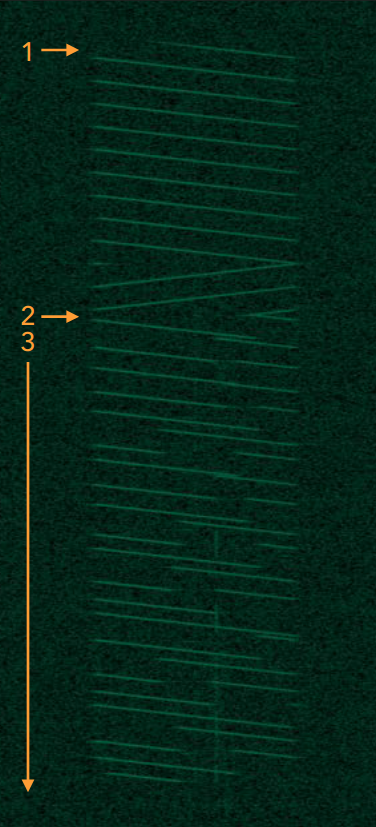
\includegraphics[width=0.8\textwidth, height=6cm]{lora_signal.png} 
        \caption{ LoRa signal}
        \label{lora1}
    \end{subfigure}
    \hspace{0.5cm}%
    \begin{subfigure}{0.7\textwidth}
        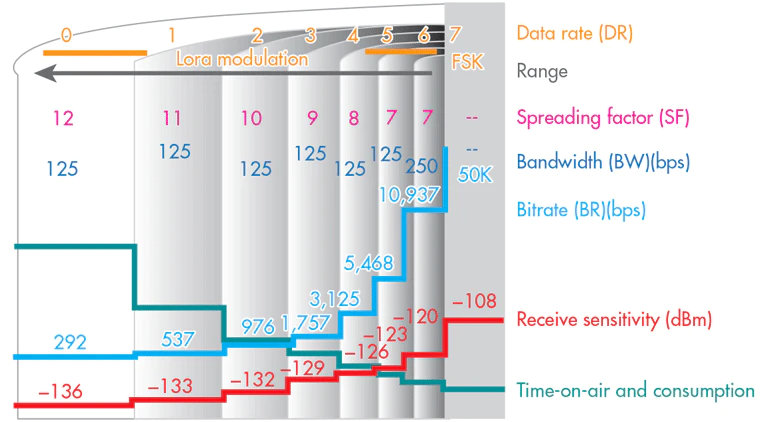
\includegraphics[width=\textwidth, height=6cm]{lora_properties.png}
        \caption{ Properties of LoRa signal}
        \label{lora2}
    \end{subfigure}
\caption[Properties of Lora signal.] {Lora signal (left) and different properties of LoRa with their effects on range, bit rate, receiver sensitivity, time on air and consumption (right). Image sources:\cite{lora_github}\cite{lora_philly}}
    \label{lora}
\end{figure}

This kind of modulation gives LoRa extreme resiliency against the interference of other radio frequency signals that might be using the same frequency band\cite{lora_article}\cite{lora_philly}.
For example, on a lower part of Figure \ref{lora1} we can see a signal with constant frequency transmitting inside the bandwidth window that the LoRa signal is using.
This kind of interference is easily filtered out by a LoRa receiver.

Size of a bandwidth window, rate of frequency change (also known as a spreading factor) and transmitting power further define LoRa signal.
With these factors, we can influence the range, power consumption and bit rate of a LoRa signal.
For example, as seen in Figure \ref{lora2}, by increasing the spreading factor we increase time on air thus giving the receiver more time to sample signal, which leads to better sensitivity but increases power consumption.

While LoRa defines the physical layer, LoRaWAN defines media access control protocol for wide area networks, which are built on top of LoRa\cite{lora_article}.
Its specification is open, so anyone can implement it.
LoRaWAN takes care of communication between end-devices and gateways and manages communication frequency bands, data rates and transmitting power.

LoRaWAN has a star of stars topology\cite{lora_article}.
Devices deployed in the field transmit messages on frequency bands that differ from region to region. 
Messages are received by gateways which relay them to the network server.
The network server displays relayed messages, decodes them and sends them to various applications.
If the same message is heard by several gateways, the server drops all duplicates.
The server also decides which gateway will send a downlink message to a specific device. 

Because LoRaWAN operates on an unlicensed ISM band, anyone can setup up their network without any licensing fees.
For some use cases, a single gateway with an internet connection is enough to provide coverage to a large number of devices.


\section{ Thermal cameras} \label{thermal_cameras}

Thermal cameras are transducers that convert infrared (IR) radiation into electrical signals, which can be used to form a thermal image.
A comparison between a normal and a thermal image can be seen on figure \ref{thermal_comparison}.
IR is an electromagnetic (EM) radiation and covers part of EM spectrum that is invisible to the human eye.
IR spectrum covers wavelengths from 780 \si{\micro\meter} to 1 \si{\milli\meter}, but only small part of that spectrum is used for IR imaging (from 0.9 \si{\micro\meter} to 14 \si{\micro\meter})\cite{thermal_book}.
We can broadly classify IR cameras into two categories: photon detectors or thermal detectors\cite{thermal_book}.
Photon detectors convert absorbed EM radiation directly into electric signals by the change of concentration of free charge carriers\cite{thermal_book}.
Thermal detectors covert absorbed EM radiation into thermal energy, raising the detector temperature\cite{thermal_book}. 
The change of the detector's temperature is then converted into an electrical signal.
Since photon detectors are expensive, large and therefore unsuitable for our use case, we will not describe them in greater detail.
\newline 

\begin{figure}[ht]
    \begin{subfigure}{0.5\textwidth}
        \centering
        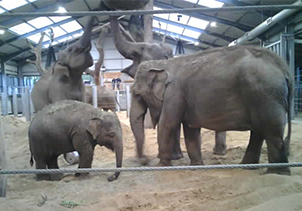
\includegraphics[width=1.0\linewidth, height=5cm]{thermal_sample_b.png} 
    \end{subfigure}
    \begin{subfigure}{0.5\textwidth}
        \centering
        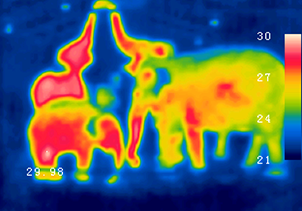
\includegraphics[width=1.0\linewidth, height=5cm]{thermal_sample_a.png}
    \end{subfigure}
    \caption[Comparison between a normal image and thermal image]{Comparison between a normal image and thermal image. Image source: Arribada Initiative\cite{thermal_comparison}}
    \label{thermal_comparison}
\end{figure}

Common examples of thermal detectors are thermopiles and microbolometers. 
Thermopiles are composed of several thermocouples.
Thermocouples consists of two different metals joined at one end, which is known as the hot junction.
The other two ends of the metals are known as cold junctions.
When there is a temperature difference between the hot and cold junctions, a voltage proportional to that difference is generated on the open ends of the metals.
To increase voltage responsivity, several thermocouples are connected in series to form a thermopile\cite{thermal_book}.
Thermopiles have lower responsivity when compared to microbolometers, but they do not require temperature stabilization\cite{thermal_book}.

Microbolometers can be found in most IR cameras today\cite{thermal_book}. 
They are sensitive to IR wavelengths of 8 to 14 \si{\micro\meter}, which is a part of the longwave infrared region (LWIR)\cite{thermal_book}.
Measuring part of a microbolometer is known as focal point array (FPA) (Figure \ref{FPA}).
FPA consists of IR thermal detectors, bolometers (Figure \ref{FPA_pixel}), that convert IR radiation into an electric signal.
Each bolometer consists of an absorber material connected to a readout integrated circuit (ROIC) over thermally insulated, but electrically conductive legs\cite{thermal_article}.
\newline

\begin{figure}[h]
    \begin{subfigure}{0.5\textwidth}
        \centering
        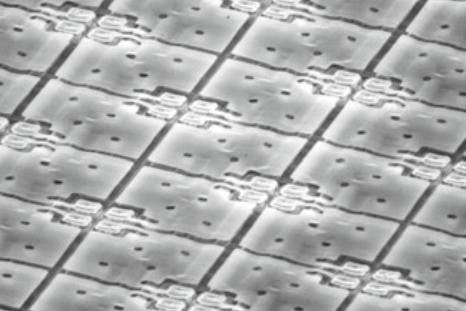
\includegraphics[width=1.0\linewidth, height=5cm]{FPA.png} 
        \caption{Focal point array}
        \label{FPA}
    \end{subfigure}
    \begin{subfigure}{0.5\textwidth}
        \centering
        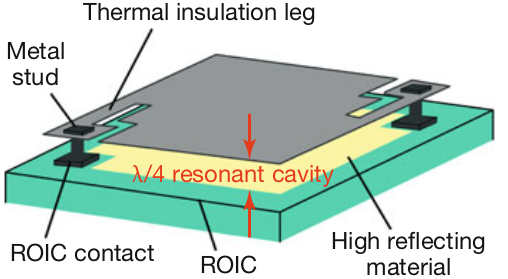
\includegraphics[width=1.0\linewidth, height=5cm]{FPA_pixel.png}
        \caption{Bolometer}
        \label{FPA_pixel}
    \end{subfigure}
    \caption[Focal point array and bolometer.] {(a) Focal point array under electronic microscope. (b) Bolometer with $\lambda /4$ resonant cavity. Image source: Vollmer, Möllmann\cite{thermal_book}}
    \label{FPA_microbolo}
\end{figure}

Absorber material is made either out of metals such as gold, platinum, titanium, or more commonly out of semiconductors such as vanadium-oxide (VOx)\cite{thermal_article}.
The important property of absorber materials is that electrical resistance changes proportionally with material's temperature\cite{thermal_book}.
When IR radiation hits absorber material, it is converted into thermal energy, which raises the absorber's temperature, thus changing its resistance.
To detect the change in resistance, ROIC applies steady-state bias current to absorber material, while measuring voltage over conductive legs\cite{thermal_book}. 

When deciding between different types of thermal cameras we are often comparing them in the terms of cost, size and image resolution.
One important property that also has to be taken into account is temperature sensitivity, also known as noise equivalent temperature difference (NETD).
NETD is measured in \si{\milli\kelvin} and tells us minimum temperature difference that can still be detected by a thermal camera.
In microbolometers, NETD is proportional to the thermal conductance of absorber material, among other factors\cite{thermal_book}.
The thermal conductance of bolometers is minimized by enclosing FPA into the vacuum chamber, thus excluding thermal convection and conduction due to surrounding gasses.
The only means of heat transfer that remain are radiant heat exchange (highly reflective material below the absorber is minimizing its radiative losses) and conductive heat exchange through supportive legs.
NETD also depends on the temperature inside the camera, higher ambient temperatures can raise the internal temperature, thus increasing NETD and noise present in the thermal image.
Today's thermopiles can achieve NETD of 100 \si{\milli\kelvin}, microbolometers 45 \si{\milli\kelvin}, while photon detectors can have NETD of 10 \si{\milli\kelvin}.
Although tens of \si{\milli\kelvin} does not seem a lot, we can see in Figure \ref{NETD} what a difference of 20 \si{\milli\kelvin} means for image resolution and noise.
\newline

\begin{figure}[ht]
    \begin{subfigure}{0.5\textwidth}
        \centering
        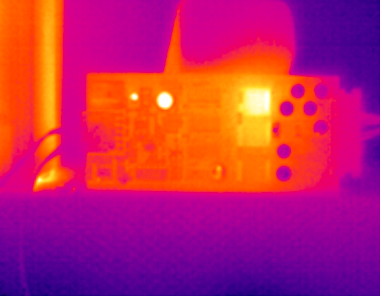
\includegraphics[width=1.0\linewidth, height=5cm]{NETD_60mk.png} 
        \caption{NETD is 60 \si{\milli\kelvin}}
        \label{NETD_60mk}
    \end{subfigure}
    \begin{subfigure}{0.5\textwidth}
        \centering
        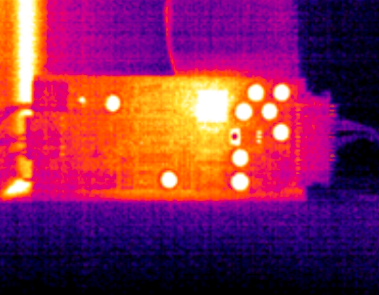
\includegraphics[width=1.0\linewidth, height=5cm]{NETD_80mk.png}
        \caption{NETD is 80 \si{\milli\kelvin}}
        \label{NETD_80mk}
    \end{subfigure}
    \caption[Comparison of images of the same object taken with cameras with different NETD values.]{Comparison of images of the same object taken with cameras with different NETD values. Low NETD values are more appropriate for object recognition. Image source: MoviTherm \cite{NETD}}
    \label{NETD}
\end{figure}


\subsection{ Choosing the thermal camera} \label{choosing_thermal}

The choice of thermal camera was made by Arribada Initiative\cite{thermal_comparison}.
They tested several different thermopiles and microbolometers while searching for desired properties.
The camera had to be relatively inexpensive and small enough so that it could be integrated into a relatively small housing.
The main property that they searched for was that elephants could be easily recognized from thermal images.
That meant that the camera needed to have decent resolution and low NETD.
Cameras were tested in Whipsnade Zoo and the Yorkshire Wildlife Park where images of elephants and polar bears could be made.

They tested two thermopile cameras (Heimann 80x64, MELEXIS MLX90640) and two microbolometer cameras (ULIS Micro80 Gen2, FLIR Lepton 2.5).
Although thermopile cameras were cheaper than microbolometer cameras, the quality of images they produced was inferior, as can be seen in Figure \ref{thermal_comparison_images}.

\begin{figure}[ht]
    \begin{subfigure}{0.5\textwidth}
        \centering
        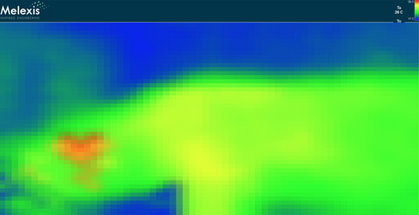
\includegraphics[width=1.0\linewidth, height=4.5cm]{thermal_comparison_a.png} 
        \label{thermal_comparison_a}
    \end{subfigure}
    \begin{subfigure}{0.5\textwidth}
        \centering
        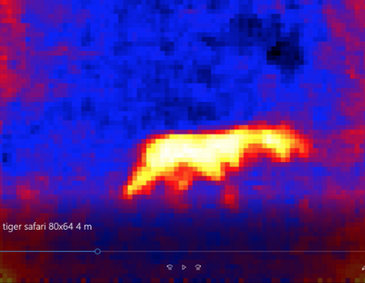
\includegraphics[width=1.0\linewidth, height=4.5cm]{thermal_comparison_b.png} 
        \label{thermal_comparison_b}
    \end{subfigure}
    \begin{subfigure}{0.5\textwidth}
        \centering
        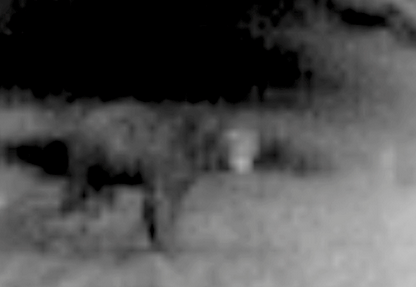
\includegraphics[width=1.0\linewidth, height=4.5cm]{thermal_comparison_c.png} 
        \label{thermal_comparison_c}
    \end{subfigure}
    \begin{subfigure}{0.5\textwidth}
        \centering
        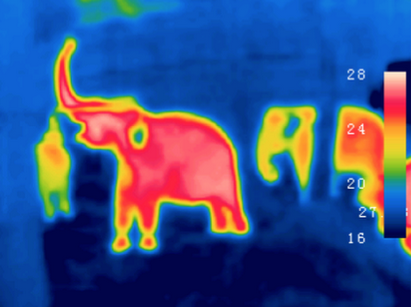
\includegraphics[width=1.0\linewidth, height=4.5cm]{thermal_comparison_d.png} 
        \label{thermal_comparison_d}
    \end{subfigure}
\caption[Comparison of image quality made by different thermal cameras.]{Comparison of image quality made by different thermal cameras, MELEXIS MLX90640 (top left), Heimann 80x64 (top right), ULIS Micro80 Gen2 (bottom left) and FLIR Lepton 2.5 (bottom right). Image source: Arribada Initiative \cite{thermal_comparison}}
    \label{thermal_comparison_images}
\end{figure}

MELEXIS MLX90640 camera had resolution of 32 x 24 pixels and NETD of 100 \si{\milli\kelvin}, while Heimann camera had resolution of 80 x 64 pixels and NETD of 400 \si{\milli\kelvin}.
It was concluded that images taken by either one of thermopile cameras could not be used for object recognition, merely only if object was present or not\cite{thermal_comparison}.

Microbolometers produced better results.
Both Ulis Micro80 and FLIR Lepton had a similar resolution, 80 x 80 and 80 x 60 respectively, but Ulis Micro80 had two times bigger NETD compared to the FLIR Lepton camera, 100 \si{\milli\kelvin} and 50 \si{\milli\kelvin}, respectively.
Images produced by FLIR Lepton were much cleaner, so it was chosen as an appropriate camera for the task.

It is important to note that FLIR Lepton, like all microbolometers, requires frequent calibration to function properly.
In temperature non-stabilized cameras small temperature drifts can have a major impact on image quality\cite{thermal_book}.
Calibration is done either by internal algorithms of the camera or by exposing the camera to a uniform thermal scene.
FLIR Lepton camera comes with a shutter, which acts as a uniform thermal signal and enables regular calibration.
Calibration in FLIR Lepton is by default automatic, triggering at startup and every 3 minutes afterward or if camera temperature drifts for more than 1.5 \si{\celsius}.

FLIR Lepton camera comes in two versions, 2.5 and 3.5.
Both cameras function the same and have exact specifications, they only differ in resolution, 3.5 has a resolution of 120 x 160, while 2.5 has 60 x 80.
In process of image collection both were used.
